\documentclass[11pt,a4paper]{article}
%%%%%%%%%%%%%%%%%%%%%%%%% Credit %%%%%%%%%%%%%%%%%%%%%%%%

% template ini dibuat oleh martin.manullang@if.itera.ac.id untuk dipergunakan oleh seluruh sivitas akademik itera.

%%%%%%%%%%%%%%%%%%%%%%%%% PACKAGE starts HERE %%%%%%%%%%%%%%%%%%%%%%%%
\usepackage{graphicx}
\usepackage{caption}
\captionsetup[table]{name=Tabel}
\captionsetup[figure]{name=Gambar}
\usepackage{tabulary}
% \usepackage{amsmath}
\usepackage{fancyhdr}
\usepackage{minted}
% \usepackage{amssymb}
% \usepackage{amsthm}
\usepackage{placeins}
% \usepackage{amsfonts}
\usepackage{graphicx}
\usepackage[all]{xy}
\usepackage{tikz}
\usepackage{verbatim}
\usepackage[left=2cm,right=2cm,top=3cm,bottom=2.5cm]{geometry}
\usepackage{hyperref}
\hypersetup{
    colorlinks,
    linkcolor={red!50!black},
    citecolor={blue!50!black},
    urlcolor={blue!80!black}
}
\usepackage{libertine}
\usepackage{libertinust1math}
\usepackage[T1]{fontenc}
\usepackage{inconsolata}

\usepackage{caption}
\usepackage{subcaption}
\usepackage{multirow}
\usepackage{psfrag}
\usepackage[T1]{fontenc}
\usepackage[scaled]{beramono}
% Enable inserting code into the document
\usepackage{listings}
\usepackage{xcolor} 
% custom color & style for listing
\definecolor{codegreen}{rgb}{0,0.6,0}
\definecolor{codegray}{rgb}{0.5,0.5,0.5}
\definecolor{codepurple}{rgb}{0.58,0,0.82}
\definecolor{backcolour}{rgb}{0.95,0.95,0.92}
\lstdefinestyle{mystyle}{
	backgroundcolor=\color{backcolour},   
	commentstyle=\color{green},
	keywordstyle=\color{codegreen},
	numberstyle=\tiny\color{codegray},
	stringstyle=\color{codepurple},
	basicstyle=\ttfamily\footnotesize,
	breakatwhitespace=false,         
	breaklines=true,                 
	captionpos=b,                    
	keepspaces=true,                 
	numbers=left,                    
	numbersep=5pt,                  
	showspaces=false,                
	showstringspaces=false,
	showtabs=false,                  
	tabsize=2
}
\lstset{style=mystyle}
\renewcommand{\lstlistingname}{Kode}
%%%%%%%%%%%%%%%%%%%%%%%%% PACKAGE ends HERE %%%%%%%%%%%%%%%%%%%%%%%%


%%%%%%%%%%%%%%%%%%%%%%%%% Data Diri %%%%%%%%%%%%%%%%%%%%%%%%
\newcommand{\stuid}{120140154}
\newcommand{\student}{\textbf{Ryan Ernanda (\stuid{})}}
\newcommand{\course}{\textbf{Sistem Operasi RB (IF2223)}}
\newcommand{\assignment}{\textbf{3}} % tugas ke...

%%%%%%%%%%%%%%%%%%% using theorem style %%%%%%%%%%%%%%%%%%%%
\newtheorem{thm}{Theorem}
\newtheorem{lem}[thm]{Lemma}
\newtheorem{defn}[thm]{Definition}
\newtheorem{exa}[thm]{Example}
\newtheorem{rem}[thm]{Remark}
\newtheorem{coro}[thm]{Corollary}
\newtheorem{quest}{Question}[section]
%%%%%%%%%%%%%%%%%%%%%%%%%%%%%%%%%%%%%%%%
\usepackage{lipsum}%% a garbage package you don't need except to create examples.
\usepackage{fancyhdr}
\usepackage[ddmmyyyy]{datetime}
\pagestyle{fancy}
\lhead{Ryan Ernanda (120140154)}
\rhead{ \thepage}
\cfoot{\textbf{Hands On 3 Docker}} % ini untuk judul tugas
\renewcommand{\headrulewidth}{0.4pt}
\renewcommand{\footrulewidth}{0.4pt}

%%%%%%%%%%%%%%  Shortcut for usual set of numbers  %%%%%%%%%%%

\newcommand{\N}{\mathbb{N}}
\newcommand{\Z}{\mathbb{Z}}
\newcommand{\Q}{\mathbb{Q}}
\newcommand{\R}{\mathbb{R}}
\newcommand{\C}{\mathbb{C}}
\setlength\headheight{14pt}

%%%%%%%%%%%%%%%%%%%%%%%%%%%%%%%%%%%%%%%%%%%%%%%%%%%%%%%555

\begin{document}
\thispagestyle{empty}
\begin{center}
	
\includegraphics[scale = 0.15]{Figure/ifitera-header.png}
	\vspace{0.1cm}
\end{center}
\noindent
% change font family for header section only
%{\fontfamily{LinuxLibertineT-OsF}\large\selectfont 
{\large
\rule{17cm}{0.2cm}\\[0.3cm]
Nama: \student \hfill Tugas Ke: \assignment\\[0.1cm]
Mata Kuliah: \course \hfill Tanggal: \today\\
\rule{17cm}{0.05cm}
\vspace{0.1cm}
}


%%%%%%%%%%%%%%%%%%%%%%%%%%%%%%%%%%%%%%%%%%%%% BODY DOCUMENT %%%%%%%%%%%%%%%%%%%%%%%%%%%%%%%%%%%%%%%%%%%%%
\begin{center}
\begin{tabular}{ |c|c| }
 \hline
 \multicolumn{2}{|c|}{\textbf{Daftar Anggota Kelompok}} \\
 \hline
 Ryan Ernanda & 120140154\\ 
 Rifan Firmansyah & 119140055 \\
 \hline
\end{tabular}
\end{center}
\section{Tujuan Hands On 3}
Tujuan dari Hands On 3 adalah untuk memahami cara kerja dari docker yang merupakan \textit{container} seperti \textit{cloud computing} yang menggunakan sub sistem dari sistem operasi lokal. Docker ini memudahkan kita dalam membuat aplikasi karena sudah tersedia \textit{virtual machine} yang lebih cepat dan efisien dalam men \textit{deploy} aplikasi ke server, daripada membangun virtual machine untuk arsiteksur server sendiri.

\section{Setup Docker}
Untuk menjalankan docker kita harus \textit{download} dan \textit{install} dahulu melalui website \href{https://www.docker.com/products/docker-desktop/}{docker.com}, disini kami \textit{install} untuk versi windows. tahap penginstallan sama seperti \textit{software} pada umumnya.
    \begin{figure}[h]
        \centering
        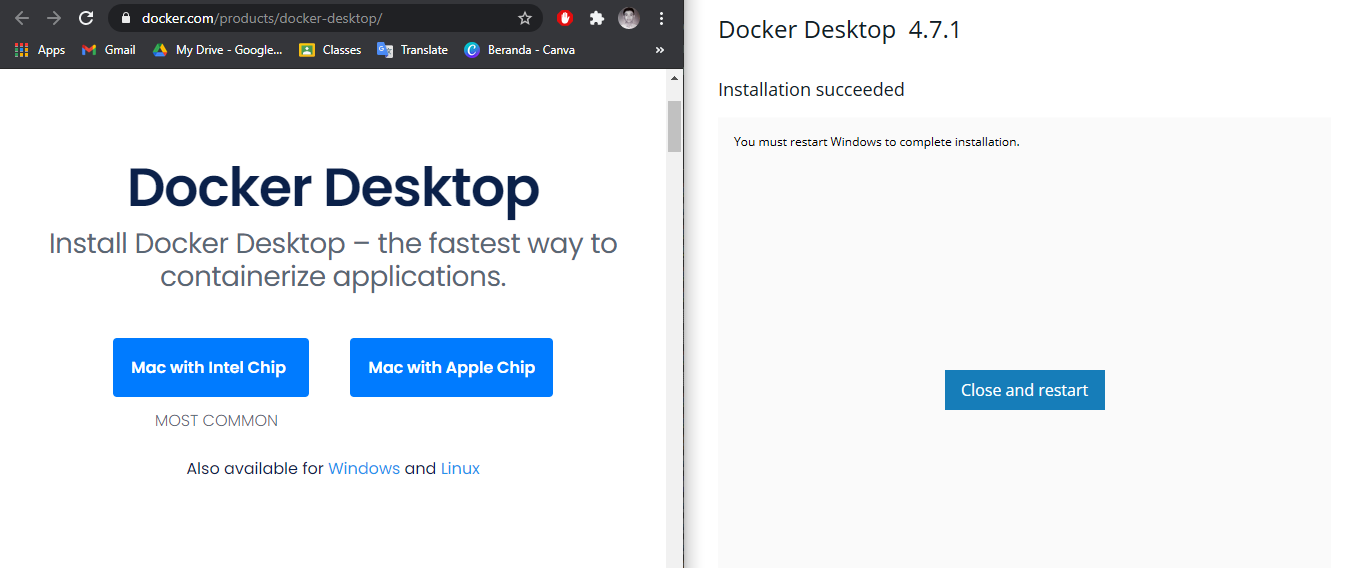
\includegraphics[width=1\textwidth]{Figure/1. install.png}
        \caption{Download dan Install Docker}
    \end{figure}
Jika sudah terinstall, docker masih belum bisa digunakan, karena docker membutuhkan wsl2. \textit{Windows Subsystem for Linux (WSL)} adalah sistem operasi yang dikembangkan oleh Microsoft supaya pengguna Windows dapat menjalankan aplikasi berbasis linux. 
\vspace{5cm}
\newline
Dalam penginstalan WSL2 bisa dilakukan manual melalui \href{https://docs.microsoft.com/en-us/windows/wsl/install-manual#step-1---enable-the-windows-subsystem-for-linux}{link} pada \textit{pop up docker}, seperti gambar dibawah.
\begin{figure}[h]
	\centering
	\begin{subfigure}[b]{0.4\textwidth}
		\centering
		\def\svgwidth{\columnwidth}
		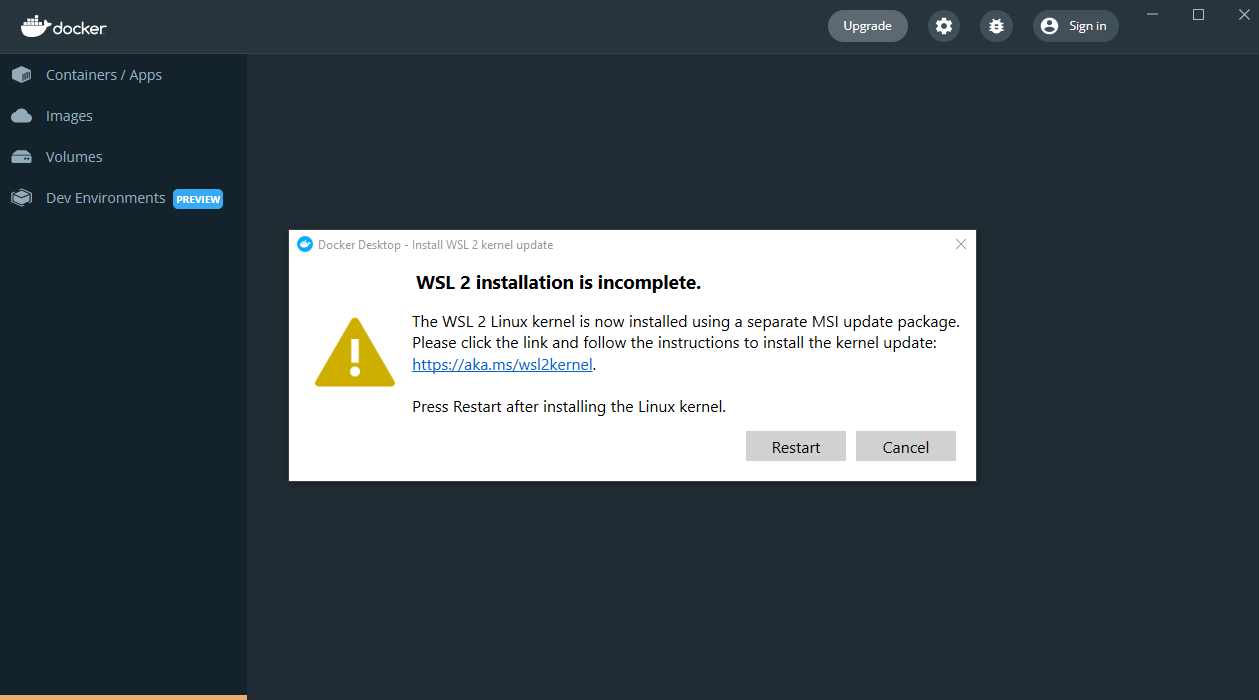
\includegraphics[width=1\textwidth]{Figure/2. pop up.png}
		\caption{Pop Up Docker}
	\end{subfigure}
	\qquad
	\begin{subfigure}[b]{0.45\textwidth}
		\centering
		\def\svgwidth{\columnwidth}
		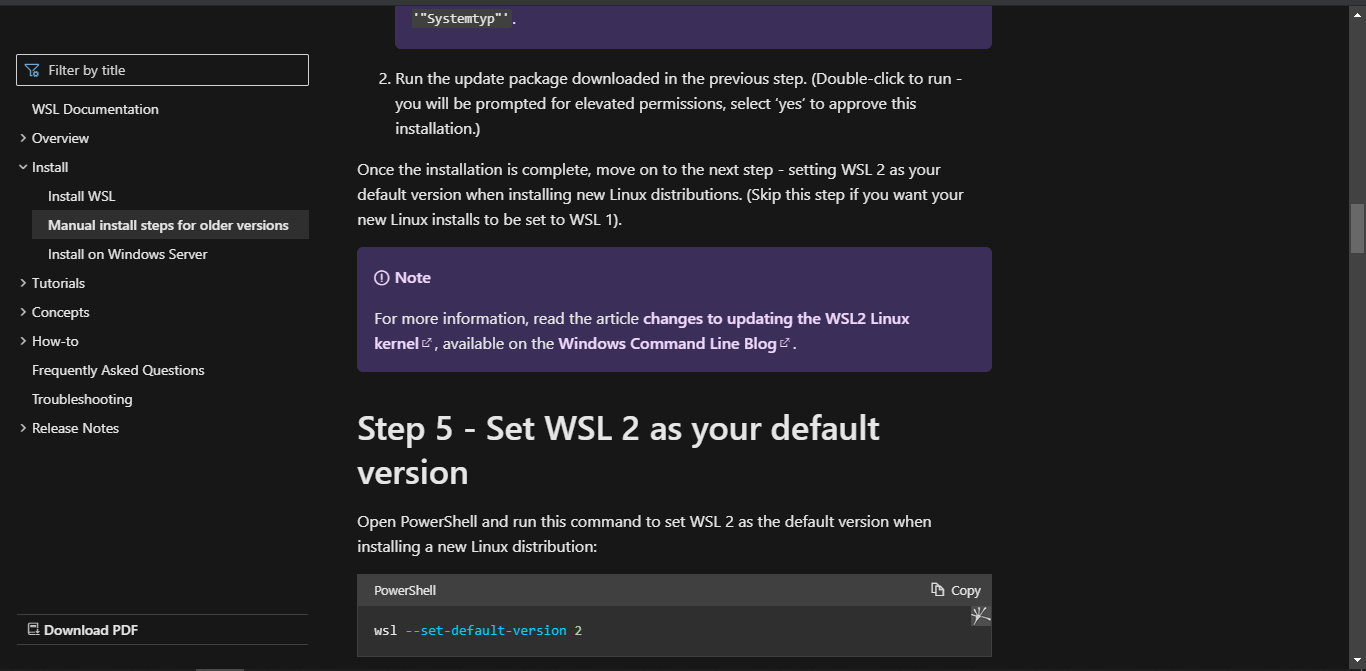
\includegraphics[width=1\textwidth]{Figure/3. wsl.png}
		\caption{Link Pop Up Docker}
	\end{subfigure}
	\caption{Install WSL2}
\end{figure}
\newline
Ikuti langkah peng-installannya dari step 1 hingga step 5, disini kami menggunakan Windows PowerShell dan berjalan sebagai admin seperti gambar dibawah ini. Setelah selesai maka diharuskan untuk \textit{restart} komputer.
 \begin{figure}[h]
     \centering
     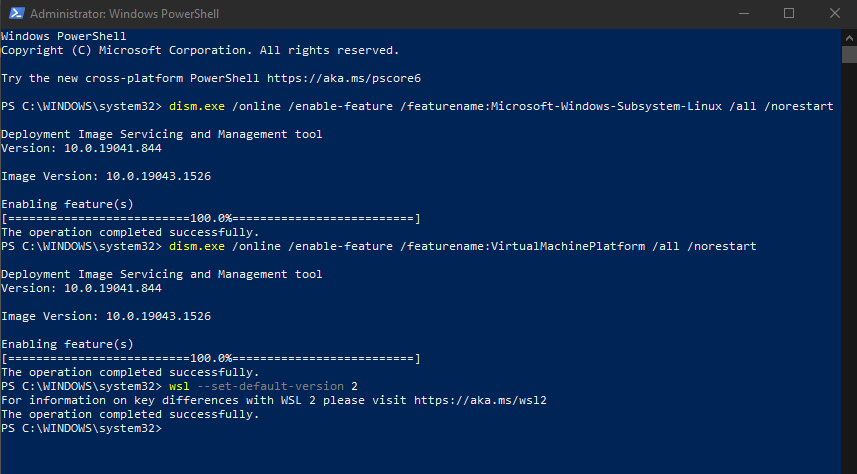
\includegraphics[width=0.5\textwidth]{Figure/4. wsl.png}
     \caption{Install WSL2 dengan Windows PowerShell}
 \end{figure}
 \newline
 Jika sudah selesai maka jalankan dan cek apakah docker sudah bisa digunakan, untuk pengecekan bisa dilihat dari logo kanan bawah dockernya, jika sudah bisa digunakan background logonya berwarna biru atau hijau yang artinya \textit{Engine Running} seperti pada gambar 4 b, jika belum maka berwarna oren atau merah seperti pada gambar 4 a.
 \begin{figure}[h]
	\centering
	\begin{subfigure}[b]{0.4\textwidth}
		\centering
		\def\svgwidth{\columnwidth}
		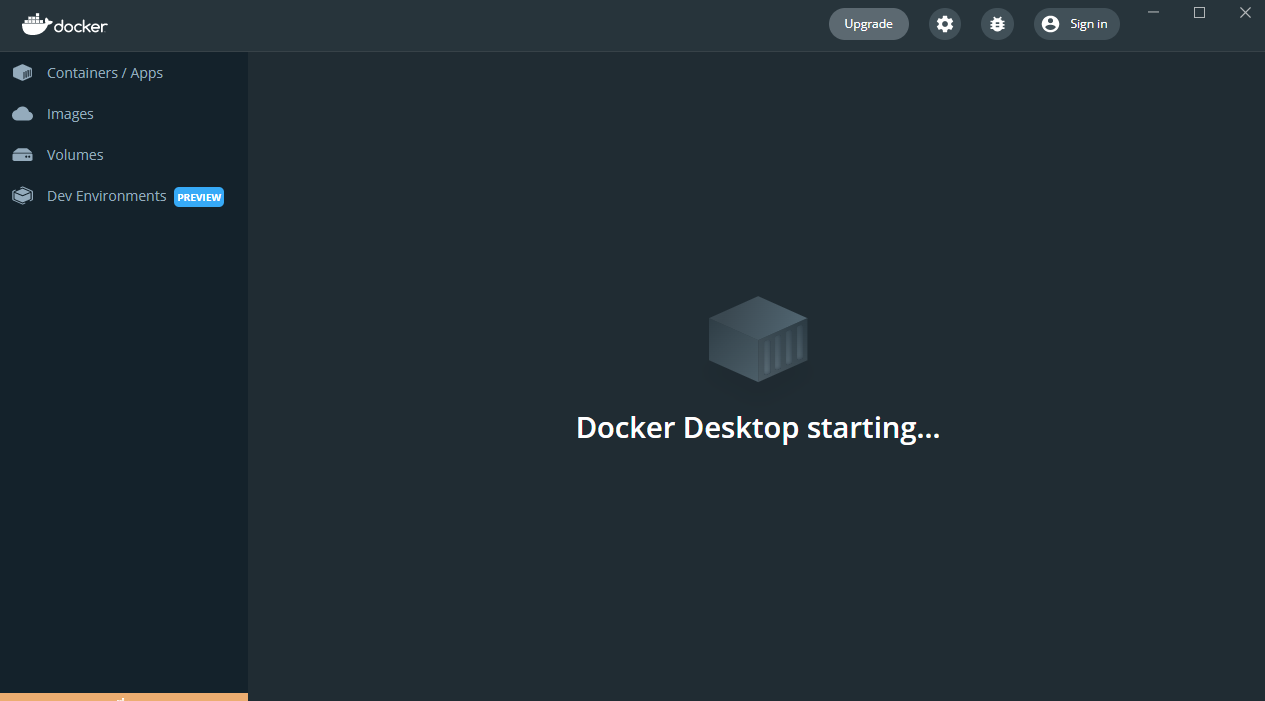
\includegraphics[width=1\textwidth]{Figure/5. wait.png}
		\caption{Docker Stop}
	\end{subfigure}
	\qquad
	\begin{subfigure}[b]{0.4\textwidth}
		\centering
		\def\svgwidth{\columnwidth}
		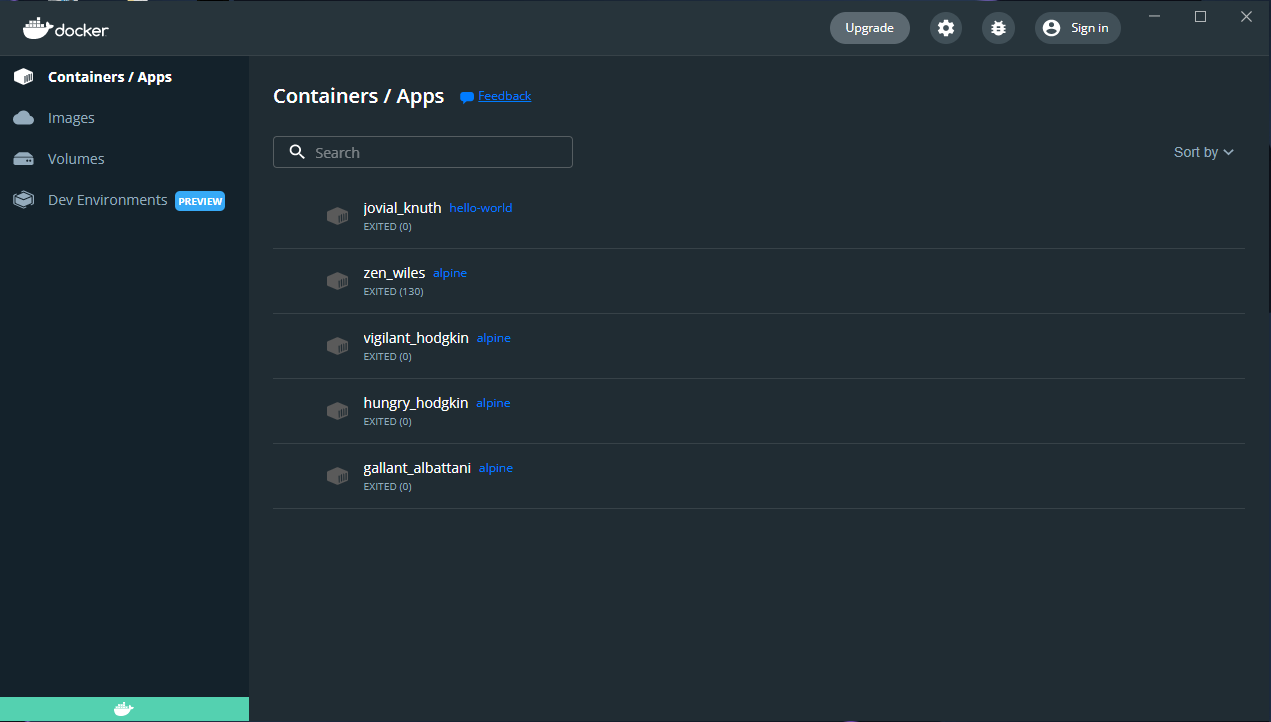
\includegraphics[width=1\textwidth]{Figure/12. docker.png}
		\caption{Docker Start}
	\end{subfigure}
	\caption{Antarmuka Docker}
\end{figure}

 \section{Menjalankan Container}
 \subsection{Hello-world}
 Untuk pertama kali menjalankan docker kami mencoba \textit{hello world} menggunakan \textit{Windows PowerShell} dengan docker command sebagai berikut, dan akan mengeluarkan seperti pada gambar 5.
 \begin{lstlisting}
 docker run hello-world\end{lstlisting}
 \begin{figure}[h]
     \centering
     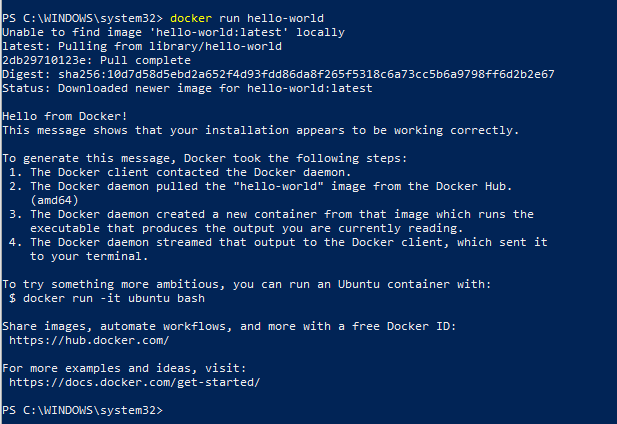
\includegraphics[width=0.6\textwidth]{Figure/6, helloworld.png}
     \caption{Docker Hello-World}
 \end{figure}
 \subsection{Alpine Linux}
 Buka \textit{Windows PowerShell} atau \textit{Command Prompt} dan mulai membuat container baru dengan docker command berikut
 \begin{lstlisting}
 docker run -it alpine sh\end{lstlisting}
 command diatas berfungsi untuk membuat container baru dengan cara mengambil images alpine dan sh, sh disini berguna untuk user agar dapat mengakses shell linux secara langsung.
 \begin{figure}[h]
     \centering
     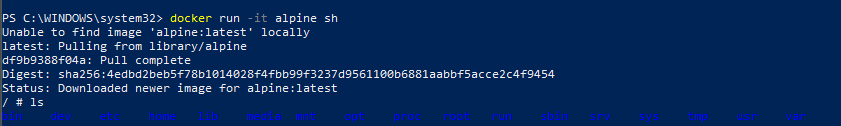
\includegraphics[width=1\textwidth]{Figure/7. create container.png}
     \caption{Pull Images dan Create Container}
 \end{figure}
 \newline
 Setelah command tersebut berhasil, container tersebut bisa di cek dengan command ls, ls disini fungsinya sama seperti \textit{syntax} di linux. Untuk nama container ini bersifat random seperti gambar diatas. Nama container bisa diubah sesuai dengan keinginan kita dengan command berikut
 \begin{lstlisting}
 docker run -it -e NAME = Ryan alpine sh\end{lstlisting}
 \newpage
 \subsection{Docker Images}
 Setelah \textit{pull} container tersebut berhasil, selanjutnya yaitu mengecek \textit{image} apa saja yang sudah pernah dilakukan \textit{pull} dengan command berikut
 \begin{lstlisting}
 docker images\end{lstlisting}
 \begin{figure}[h]
     \centering
     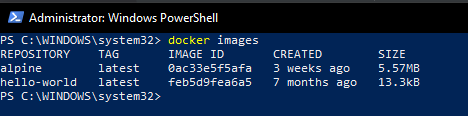
\includegraphics{Figure/8. images.png}
     \caption{Docker Images}
 \end{figure}
 Selanjutnya memunculkan proses sistem container yang telah terisolasi. hal ini menunjukkan bahwa container merupakan proses yang menjalankan Host dimana Host tersebut berupa local. Ketika docker run dieksekusi, container yang sudah dijalankan akan terisolasi karena memiliki file sistem dan jaringan sendiri. Untuk menjalankan \textit{container docker alpine} dengan urutan image ini, bisa menggunakan command berikut
 \begin{lstlisting}
 docker run alpine ls -l\end{lstlisting}
 \begin{figure}[h]
     \centering
     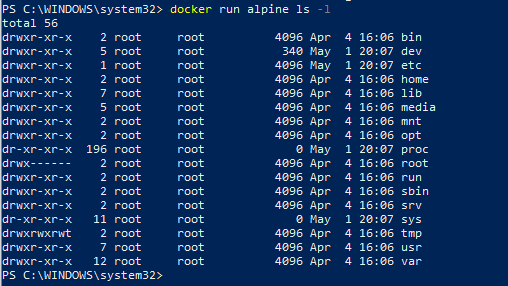
\includegraphics[width=0.8\textwidth]{Figure/9. show proses container.png}
     \caption{Docker Run Alpine Ls -l}
 \end{figure}
 berikutnya kami menampilkan kalimat pada \textit{windows powershell} dengan \textit{command docker run alpine} dan tambahan \textit{echo}, \textit{echo} disini sama fungsinya seperti linux. berikut commandnya
  \begin{lstlisting}
 docker run echo "Ini Kalimat"\end{lstlisting}
 \begin{figure}[h]
     \centering
     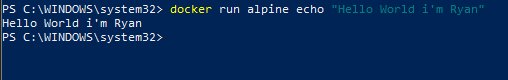
\includegraphics[width=0.7\textwidth]{Figure/10. helloworld.png}
     \caption{Hello World I'm Ryan}
 \end{figure}
 Terakhir menampilkan container yang sudah dijalankan sebelumnya dengan command
 \begin{lstlisting}
 docker ps -a\end{lstlisting}
 \begin{figure}[h]
     \centering
     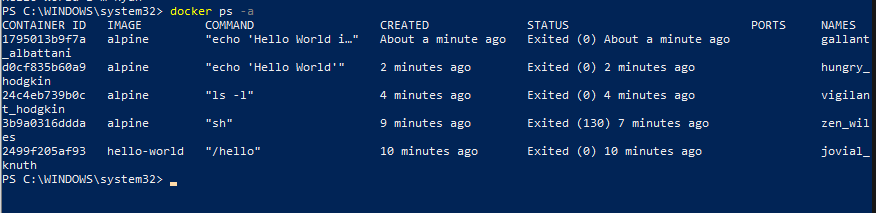
\includegraphics[width=1\textwidth]{Figure/11. perintah yang dah pernah.png}
     \caption{Docker Ps -a}
 \end{figure}
 Jika ingin lebih mudah bisa dilihat melalui aplikasi dockernya langsung seperti gambar dibawah ini
 \begin{figure}[h]
     \centering
     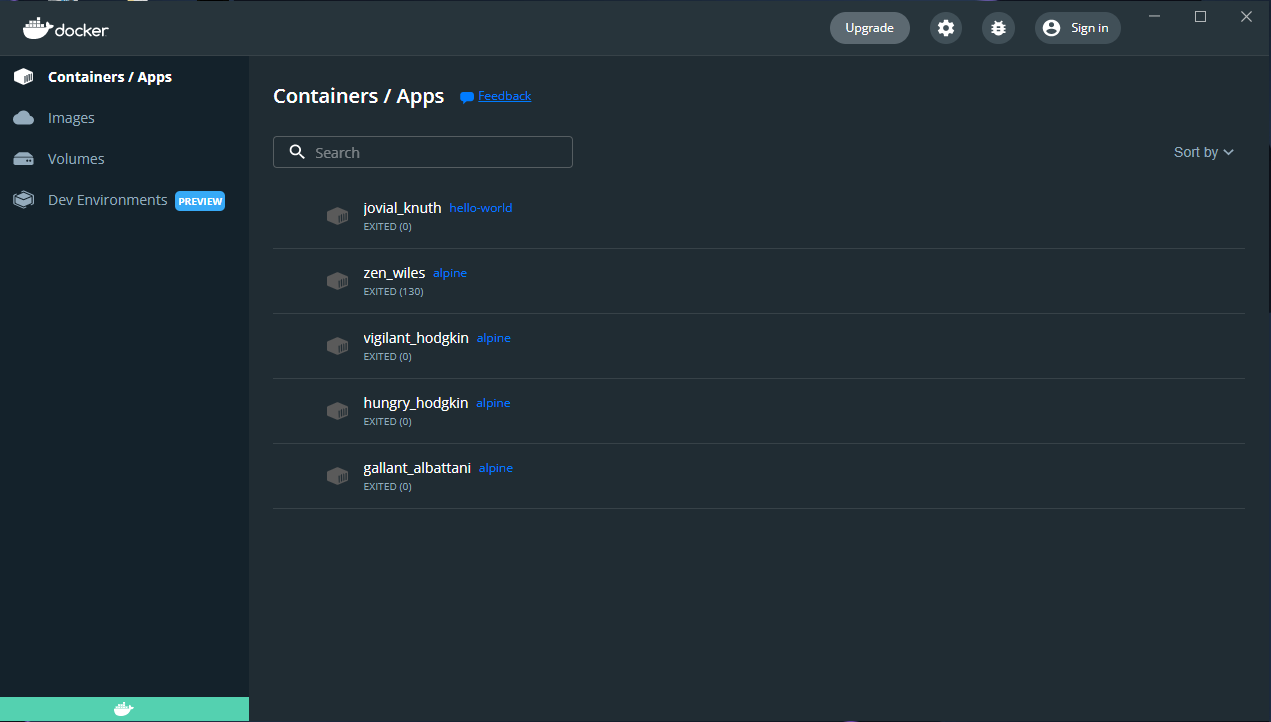
\includegraphics[width=0.7\textwidth]{Figure/12. docker.png}
     \caption{Antarmuka Docker}
 \end{figure}
 
 \section{Pertanyaan Hands On 3}
\subsection{Apa Itu Docker}
Docker merupakan sebuah layanan aplikasi yang disebut dengan container yang berfungsi untuk menyediakan suatu kemampuan untuk mengemas dan menjalankan sebuah aplikasi dalam sebuah lingkungan terisolasi. Dengan adanya isolasi dan keamanan yang memadai, memungkinkan  untuk menjalankan banyak container di waktu yang bersamaan pada host tertentu. Dan juga docker dapat membantu untuk meningkatkan produktivitas dari developer dalam membuat perangkat lunak yang berkualitas\cite{dewaweb}.

\subsection{Apa Fungsi Dari Docker Run}
Perintah docker run digunakan untuk menjalankan proses dalam container yang terisolasi. Images yang terdapat dalam container akan dieksekusi sesuai dengan konfigurasi yang akan dibuat. Ketika perintah docker run dijalankan, image container akan dieksekusi seolah-olah Anda sedang menjalankan  aplikasi. Biasanya, memiliki beberapa port yang terbuka sehingga aplikasi  di dalam container yang sedang berjalan dapat  diakses dari luar container 

\subsection{Apa Yang Dimaksud Dengan Container}
Docker container merupakan environment untuk mengemas aplikasi yang mencakup system tools, library, code, runtime dan konfigurasi.

\subsection{Apa yang terjadi ketika perintah docker ps -a dilakukan}
\textit{docker ps -a} merupakan sebuah command docker untuk menampilkan semua data container yang pernah dibuat. Untuk \textit{"ps-a"} menampilkan \textit{container id} hingga \textit{names} seperti gambar dibawah
\begin{figure}
    \centering
    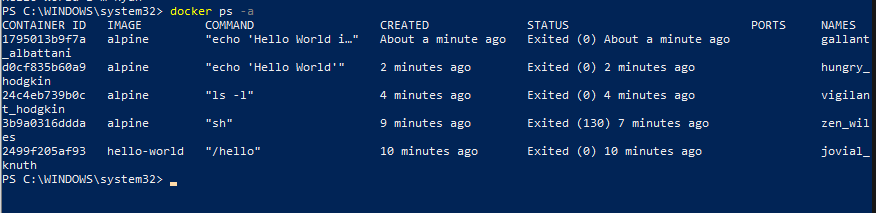
\includegraphics[width=1\textwidth]{Figure/11. perintah yang dah pernah.png}
    \caption{Docker Ps-a}
\end{figure}

\subsection{Apa yang terjadi ketika perintah docker run -it dilakukan}
\textit{Docker run -it} merupakan sebuah command docker untuk mengalokasi sebuah \textit{pseudo-TTY} atau bentuk komunikasi dua arah antara komputer utama dengan ruang yang terisolasi dengan membuat sebuah \textit{interactive bash shell} pada container. perintah yang digunakan sebagai berikut
\begin{lstlisting}
docker run -it\end{lstlisting} 

\subsection{Apa yang dimaksud dengan Images}
Docker image adalah kumpulan file yang berisi informasi untuk membangun sebuah container.

\subsection{Apa yang dimaksud dengan daemon}
Docker daemon adalah tempat pengelolaan Docker image, container, network, dan volume. Daemon menyediakan command-line-interface (CLI) sisi client agar user dapat berinteraksi dengan daemon lewat Docker API. Bertugas menerima request dari Docker API yang akan diproses selanjutnya oleh sistem.

\section{Kesimpulan}
Yang dapat Kami simpulkan dari hasil Tugas HandsOn 3 ini yaitu \textit{Docker} berfungsi untuk memudahkan \textit{developer} dalam melakukan \textit{build, shipping} dan \textit{run} pada sebuah \textit{container} melalui infrastruktur dari PC \textit{developer}.\textit{Resource} dibutuhkan dalam membuat aplikasi ini hanya sedikit dan sangat berguna untuk \textit{developer}.
\newpage
\bibliographystyle{IEEEtran}
\bibliography{Referensi}
\end{document}